\documentclass[Ex4_Zusammenfassung.tex]{subfiles}

\begin{document}
\section{Tiefinelastische Streuung}
\textbf{von S\o{}ni \& Martina}\\

Nun wollen wir uns mit der Frage beschäftigen, wie die Struktur innerhalb eines Kernes aussieht. Für Energien groß genug dringen die Streuteilchen in den Kern ein. Somit lässt sich die tiefinelastische Streuung als elastische Streuung an \textbf{Partonen} = ''Konstituenten des Nukleus'' beschreiben.
\begin{figure}[H]
	\centering
	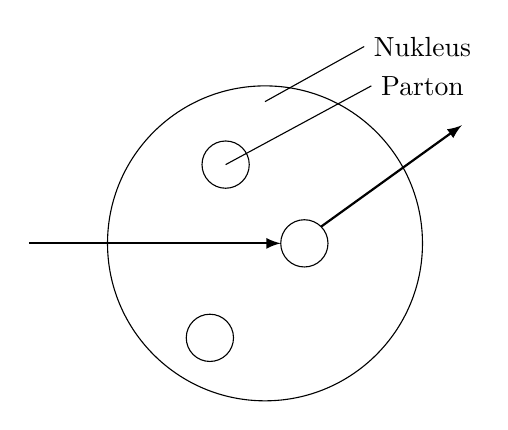
\begin{tikzpicture}
	%defs
	\def\ra{0.3cm}
	%nodes
	\node at (2,2.5) (nuk) {Nukleus};
	\node at (2, 2) (par) {Parton};
	%shapes
	\draw (0,0) circle (2cm);
	\draw (0.5,0) circle (\ra);
	\draw (-0.5,1) circle (\ra);
	\draw (-0.7,-1.2) circle (\ra);
	%lines
	\draw (nuk.west) -- (0,1.8);
	\draw (par.west) -- (-0.5,1);
	\draw [thick, ->, >=latex] (-3,0) -- (0.2,0);
	\draw [thick, ->, >=latex] (0.712,0.212) -- (2.5,1.5);
	\end{tikzpicture}
	\caption{Schema der elastischen Streuung an Partonen}
\end{figure}

Bei festen $q^2$ und $\nu$ kann $\tan^2 \frac{\theta}{2}$ auf der X--Achse und $2W_1\lp q^2,\nu\rp \tan^2 \frac{\theta}{2} + W_2\lp q^2,\nu\rp$ auf der Y--Achse aufgetragen werden. Daraus lässt sich folgender Zusammenhang schreiben:
\begin{equation}
	y(x) = 2W_1x+W_2
\end{equation}

Wir wollen aus Messungen die dimensionslosen Strukturfunktionen $F$ bestimmen:
\begin{align}
	F_1\lp x,q^2\rp &= Mc^2 W_1\lp q^2,\nu\rp\\
	%%
	F_2\lp x,q^2\rp &= \nu W_2\lp q^2,\nu\rp
\end{align}
wobei $\nu$ den Energieübertrag (da inelastische Streuung; bei elastischer Streuung nur Impulsübertrag) und $x$ die Bjorken'sche Skalenvariable (Inelastizität der Streuung) beschreiben. $x$ ist definiert durch:
\begin{equation}
	x = \frac{-q^2}{2M\nu}
\end{equation}

\subsection*{Wirkungsquerschnitt}
Für den Wirkungsquerschnitt gilt
\begin{equation}
	\derive{^2\sigma}{\lp q^2\rp \md \nu} = \frac{4 \pi \alpha^2}{q^4} \frac{E^\prime}{E\nu}\lp F_2 \cos^2 \frac{\theta}{2} + \frac{2\nu}{M}F_1\sin^2 \frac{\theta}{2} \rp 
\end{equation}
Mit den Beziehungen $\cos^2 \frac{\theta}{2} = 1 + \frac{q^2}{\Delta E E^\prime}$, $\frac{\md \nu}{\nu} = \frac{\md x}{x}$ und $y=\frac{\nu}{E}$ (relativer Energieübertrag) folgt:
\begin{equation}
	\derive{^2 \sigma}{\lp q^2\rp \md x} = \frac{4\pi \alpha^2}{q^4} \lp \lp 1-y\rp \frac{F_2}{x} + y^2 F_2\rp
\end{equation}

\subsection*{Quasielastische Streuung an punktförmigen Teilchen}
Bei der quasielastischen Streuung an punktförmigen Teilchen hängen $F_1$ und $F_2$ nicht von $q^2$ ab, da die Formfaktoren bei punktförmiger Ladungsverteilung konstant sind. 
\begin{figure}[H]
	\centering
	\begin{tikzpicture}
		\begin{feynman}
			%vertices
			\vertex (i1);
			\vertex [right=of i1] (a1temp);
			\vertex [below=0.5 cm of a1temp] (a1);
			\vertex [right=of a1temp] (o1);
			\vertex [below=of a1] (a2);
			\vertex [below=2.5cm of i1] (i2);
			\vertex [below=0.3cm of i2] (i3);
			\vertex [below=0.3cm of i3] (i4);
			\vertex [below=3cm of o1] (o2) {$m$};
			\vertex [below=1.8cm of o1] (o3);
			\vertex [below=0.3cm of o3] (o4);
			%diagram
			\diagram* {
				(i1) -- [fermion, edge label=$e$] (a1) -- [fermion, edge label=$e$] (o1),
				(a1) -- [photon, edge label=$q$] (a2),
				(i2) -- [fermion, edge label=$zP$] (a2) -- [fermion] (o2.west),
				(i3) -- [fermion] (o3),
				(i4) -- [fermion] (o4)
				};
			%decorations
			\draw [decoration={brace, mirror, raise=0.2cm}, decorate] (i2.north)  -- (i4.south) node [pos=0.5, left, xshift=-0.3cm, text width=1.5cm] {Nukleon Masse M Impuls P};
		\end{feynman}
	\end{tikzpicture}
	\caption{Schema der quasielastischen Streuung an Partonen. $m$ ist die invariante Masse des Partons, $q$ der 4er--Impulsübertrag}
\end{figure}
Im Bezugssystem, in dem der Impuls des Protons (Nukleons) $P \rightarrow \infty$, gilt:

\begin{table}[H]
	\centering
	\begin{tabular}{cc}
		Proton & Parton \\ 
		\hline 
		$P$ & $zP$ \\ 
		$E$ & $zE$ \\ 
	\end{tabular}
\end{table}
wobei $z \in \left[ \left. 0,1\right) \right. $ ein Lorentzskalar ist. Dann folgt für die invariante Masse des Partons
\begin{equation}\label{eq:partonmasse}
	m^2 = \lp zP + q \rp^2 = \underbrace{z^2P^2}_{m^2} + q^2 + 2zPq
\end{equation}
woraus sich für $z$ Folgendes ergibt
\begin{equation}
	z = -\frac{q^2}{2Pq}
\end{equation}
wobei hier $P$ den 4er--Impuls und $q$ den 4er--Impulsübertrag darstellt. Um \ref{eq:partonmasse} besser zu verstehen, betrachten wir nun die 4er--Impulserhaltung und $P\rightarrow \infty$:
\begin{align}\label{eq:impulse1}
	\rom{1}&: P_e + zP = P_{\rom{1}}\\ \label{eq:impulse2}
	\rom{2}&: P_e^\prime + zP+q = P_{\rom{2}}
\end{align}
Hier beschreiben $P_e$ und $P_e^\prime$ die (4er--)Impulse des Elektrons vor und nach der Streuung und $zP$ den Anteil des Gesamtimpulses $P$ den das Parton besitzt. Aus der 4er--Impulsquadraterhaltung und $P^2 = \braket{P,P}=m^2$ folgt
\begin{equation}
	P_{\rom{1}}^2 = P_{\rom{2}}^2 \stackrel{!}{=} m^2
\end{equation}
Setzen wir nun die Gleichungen \ref{eq:impulse1} und \ref{eq:impulse2} ein:
\begin{align*}
	\lp P_e + zP \rp^2 &= \lp P_e^\prime + zP+q\rp^2 \stackrel{!}{=} m^2\\
	\intertext{Mit der Bedingung P\rightarrow\infty\ sind}
	P_e,\ P_e^\prime,\ q &\ll P\\
	\intertext{und somit}
	(zP)^2 = (zP)^2 \stackrel{!}{=} m^2
\end{align*}
Das 4er--Impulsquadrat ist außerdem
\begin{align}
	P^2 &= \fourvec{E=\sqrt{m^2 + \lvert \vec{p}\rvert^2}}{p_1}{p_2}{p_3}^2_\text{Minkowski}\\
	&= m^2 + \lvert \vec{p} \rvert^2 \underbrace{-p_1^2 - p_2^2 -p_3^2}\\
	&= m^2 + \lvert \vec{p} \rvert^2 \kern 1.5em -  \lvert \vec{p} \rvert^2\\
	&= m^2 
	\intertext{was zu zeigen war.}
\end{align}
Hier sieht man sehr schön, dass Gesamtviererimpulsquadrate in abgeschlossenen Systemen \textbf{lorentzinvariant} und \textbf{erhalten} sind.\\

Da $z$ ein Lorentzskalar ist, ist das Bezugssystem beliebig:
\begin{equation*}
	P = \lp M,\ \vec{0} \rp \text{ und } q=\lp \nu,\ \vec{q} \rp \text{ und somit } Pq=M\nu
\end{equation*}
Daraus folgt nun wiederrum 
\begin{equation}
	z=x=-\frac{q^2}{2M\nu}
\end{equation}
Ein Photon mit $x$ wird von einem Parton mit Impulsanteil $x=z$ absorbiert. Im Laborsystem gilt: 
\begin{equation}
	z=x=-\frac{q^2}{2M\nu}=\frac{2m\nu}{2M\nu}=\frac{m}{M}
\end{equation}
Durch den Vergleich der Wirkungsquerschnitte von elastischer und inelastischer Streuung von Spin $\nicefrac{1}{2}$--Teilchen folgt
\begin{align}
	\intertext{für die elastische Streuung:}
	\derive{\sigma}{\lp q^2\rp} &= \frac{4 \pi \alpha^2}{q^4} \frac{E^\prime}{E} \lp \cos^2\lp \frac{\vartheta}{2}\rp + \frac{q^2}{2m^2} \sin^2\lp \frac{\vartheta}{2}\rp \rp\\
	\intertext{und für die inelastische Streuung:}
	\derive{^2 \sigma}{\lp q^2\rp \md x} &= \frac{4 \pi \alpha^2}{q^4} \frac{E^\prime}{E} \lp F_2 (x) \cos^2 \lp \frac{\vartheta}{2} \rp+ \frac{q^2}{2M^2x^2} 2xF_1(x) \sin^2 \lp \frac{\vartheta}{2} \rp \rp \frac{1}{x}
\end{align}
Aus Koeffizientenvergleich folgt:
\begin{equation}
	F_2(x) = \sum_i e_i^2 x f_i(x)
\end{equation}
mit der Wahrscheinlichkeit $f_i(x)\md x$, das Parton $i$ mit der Ladung $e_i$ im Impulsintervall $\left[ x,x+\md x \right]$ anzutreffen. Überdies folgt aus dem Koeffizientenvergleich auch:
\begin{equation}
	\frac{2xF_1(x)}{F_2(x)}=1
\end{equation}
Bei großen $q^2$--Werten ist $F_2$ doch von $q^2$ abhängig, da das Modell die Wechselwirkung von Quarks und Gluonen vernachlässigt (z.B. Streuung an Seequarks).

\begin{figure}[H]
	\centering
	\begin{tikzpicture}
		\begin{feynman}
			%verices
			\vertex (i1);
			\vertex [right=of i1] (a1temp);
			\vertex [below=0.5cm of a1temp] (a1);
			\vertex [right=of a1temp] (o1);
			\vertex [below=of a1] (a2);
			\vertex [left=0.5cm of a2] (a2temp);
			\vertex [below=0.1cm of a2temp] (a3);
			\vertex [below=of a3] (a4);
			\vertex [below=of o1] (o5) {$q$};
			\vertex [below=of o5] (o6) {$\overline{q}$};
			\vertex [left=of a4] (i2);
			\vertex [below=0.3cm of i2] (i3);
			\vertex [below=0.3cm of i3] (i4);
			\vertex [right=of a4] (o2temp);
			\vertex [right=0.5cm of o2temp] (o2);
			\vertex [below=0.3cm of o2] (o3);
			\vertex [below=0.3cm of o3] (o4);
			\vertex [above=0.3cm of i1] (t1temp);
			\vertex [left=1cm of t1temp] (t1);
			\vertex [right=5cm of t1] (t2);
			
			%shapes
			\draw (i3) ellipse (0.2cm and 0.6cm);
			\draw [->, >=latex] (t1) -- (t2) node [midway, above] {$t$};
			\draw [decoration={brace, mirror}, decorate] (o6.south east) -- (o5.north east) node [pos=0.5, right] {Seequarks};
			
			%diagram
			\diagram* {
				(i1) -- [fermion, edge label=$e^-$] (a1) -- [fermion, edge label=$e^-$] (o1),
				(a1) -- [photon, edge label=$\gamma$] (a2),
				(a4) -- [gluon, edge label=$g$] (a3) -- (a2) -- [fermion] (o5),
				(a3) -- [anti fermion] (o6),
				(i2) -- [fermion] (a4) -- [fermion] (o2),
				(i3) -- [fermion] (o3),
				(i4) -- [fermion] (o4)
				};
		\end{feynman}
	\end{tikzpicture}
	\caption{Feynman--Diagramm der Streuung eines Elektrons an einem Seequark}
\end{figure}
Die angepasste $F_2$ ist dann
\begin{equation}
	F_2 = \sum_{a=u,d,s} e_a^2 x f_a(x) + \underbrace{e_a^2 x f_{\overline{a}}(x)}_{\text{Antiquarks}}
\end{equation}
Verteilung von Quark/Antiquark--Verteilung mit Elektron-- oder Myonstreuung nicht möglich, daher wird Neutrino--Nukleon--Streuung verwendet.
\begin{figure}[H]
	\centering
	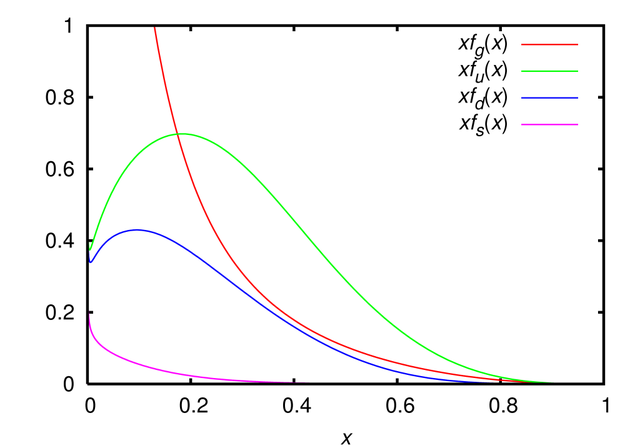
\includegraphics[scale=0.3]{640px-CTEQ6_parton_distribution_functions.png}
	\caption{Quark--Antiquark Verteilung. Für hohe $q^2$ verschiebt sich der Valenzquarkanteil (blau) nach links.}
\end{figure}
Aus der Neutrino--Nukleon--Streuung lernt man, dass im Bereich mit dominantem Valenzquarkanteil $(x>0.3)$ gilt:
\begin{equation}
	\frac{F_2^{\text{ep}} + F_2^{\text{en}}}{F_2^{\nu\text{p}} + F_2^{\nu\text{n}}} = \frac{e_u^2+e_d^2}{2} = \frac{5}{18}
\end{equation}
Daran erkennt man natürlich sofort, dass Partonen $\nicefrac{1}{3}$--wertige Ladungen besitzen, wodurch man Partonen als Quarks identifizieren kann. 
\end{document}
